

\documentclass[10pt,journal,compsoc]{IEEEtran}
\usepackage{graphicx}
\usepackage{hyperref}
\usepackage{multirow}
\usepackage[normalem]{ulem}
\useunder{\uline}{\ul}{}
\usepackage{caption}

\ifCLASSOPTIONcompsoc
  % IEEE Computer Society needs nocompress option
  % requires cite.sty v4.0 or later (November 2003)
  \usepackage[nocompress]{cite}
\else
  % normal IEEE
  \usepackage{cite}
\fi


\ifCLASSINFOpdf
  % \usepackage[pdftex]{graphicx}
  % declare the path(s) where your graphic files are
  % \graphicspath{{../pdf/}{../jpeg/}}
  % and their extensions so you won't have to specify these with
  % every instance of \includegraphics
  % \DeclareGraphicsExtensions{.pdf,.jpeg,.png}
\else
  % or other class option (dvipsone, dvipdf, if not using dvips). graphicx
  % will default to the driver specified in the system graphics.cfg if no
  % driver is specified.
  % \usepackage[dvips]{graphicx}
  % declare the path(s) where your graphic files are
  % \graphicspath{{../eps/}}
  % and their extensions so you won't have to specify these with
  % every instance of \includegraphics
  % \DeclareGraphicsExtensions{.eps}
\fi

\hyphenation{op-tical net-works semi-conduc-tor}


\begin{document}

\title{Semantic Web Ontologies Pertaining to\\ Heterogeneity and Social Networks}

\author{Daniela~Martignani, %~\IEEEmembership{Member,~IEEE,}
        Peter~Miele,%~\IEEEmembership{Fellow,~OSA,}
        and~Jennifer~Shaska %,~\IEEEmembership{Life~Fellow,~IEEE}% <-this % stops a space
\IEEEcompsocitemizethanks{\IEEEcompsocthanksitem Authors are graduate students in the Department
of Computer Science and Engineering, Oakland University, Rochester,
MI, 48309.\protect\\
\IEEEcompsocthanksitem dmartign@oakland.edu,pamiele@oakland.edu,jlshaska@oakland.edu}% <-this % stops an unwanted space
\thanks{Manuscript submitted April 7, 2016}}

%\markboth{Journal of \LaTeX\ Class Files,~Vol.~14, No.~8, August~2015}%
%{Shell \MakeLowercase{\textit{et al.}}: Bare Demo of IEEEtran.cls for Computer Society Journals}

\IEEEtitleabstractindextext{%
\begin{abstract}
In this paper we will summarize three current  documents on how ontologies can be used to navigate and combine social networks to facilitate decisions on which meaning or instance of a concept a user wants to see. A common problem amongst this domain is linking concepts between ontologies if those ontologies use different semantics for the same concept or the same semantics for different concepts, techniques are evolving to solve this problem. We will also cover a summary of various ontology description languages and how they interact in semantic web for various uses. These techniques and ontology languages can be used when querying social networks to find relations to narrow the search down to those that are relevant to the current user. 
\end{abstract}


\begin{IEEEkeywords}
 Ambiguity, Ontology, Redundancy,  Semantic Web, Social Network,
\end{IEEEkeywords}}


\maketitle



\IEEEdisplaynontitleabstractindextext

\IEEEpeerreviewmaketitle



\IEEEraisesectionheading{\section{Introduction}\label{sec:introduction}}

\IEEEPARstart{T}{he} semantic web is a means of using the world wide web to create a method of sharing data between computers so that a machine can query and infer knowledge from existing information. In this paper we will cover three existing sources of information on the semantic web. 

Currently the web is not organized in a manner in which information can be processed easily by a machine; instead it is structured to be utilized by humans who can parse and extract information that is presented in an unorganized manner. Semantic web provides a means of organization that structures information in a simple format that can easily be parsed and utilized by a machine to handle user queries, and create inferences based on formal logic systems.

Sections 2.1 and 2.2 will cover the data format of the semantic web and why it is structured the way it is in comparison to well-known formats. This will cover the Resource Description Framework (RDF), the Resource Description Framework schema (RDFs), and the Web Ontology Language (OWL) and how they relate to well-known data formats like EXtensible Markup Language (XML), Unified Modeling Language (UML), and Entity/Relation Modeling (E/R Modeling) of databases. This background and conceptual overview will provide a basis for understanding the underlying concepts of the semantic web so that their application can be appreciated.

Section 2.3 will cover the notions of the issues of independent actors all trying to author and use the semantic web at once with no over-arching governing body. This will go over the problem of multiple resources having the same identifier, called semantic ambiguity. We will also cover the issue of multiple authors all authoring the same resource which means query processor has to find the correct one which is semantic redundancy. Their findings indicate that you can, at better than chance rate, determine the correct resource to use when performing a search using an ambiguous term and relate that term across different ontologies.

Section 2.4 will review a paper that applies some of these concepts in the realm of social media and connecting users across social networks. This paper addresses the issue of social networks not being able to interconnect amongst the web of all social networks. This is due to the ever changing landscape of social media content and the lack of a framework that successfully integrates the different ontologies to relate all the users and content. They presented an overview of existing ontologies, such as Friend-of-a-Friend (FOAF), Semantically Interlinked Online Communities (SIOC), Simple Knowledge Organization System (SKOS), and Dublin Core (DC) and how these ontologies can be used together to build a framework and address the issue of creating a more interconnected web. A brief discussion is included of how this framework will help describe user generated content on social networks and how it relates to users.

%Once the semantic web grows and matures users will be able to be linked and identified across social networks based on the %ontologies presented by each social network. This will allow the interconnection of users across social networks and allow for a %better understanding of how people communicate and relate using social networks.


\section{Reviews of Documents}
\subsection{\textit{Social networks and the semantic web} \cite{_social_2007}}
The current version of the web contains lots of unstructured data which is easily understood by humans but not easily understood by machines.  People are naturally able to process this data due to our ability to infer new ideas based on ideas we already know, and our ability to make connections between somewhat unrelated topics.  The main goal of the Semantic Web is to have structured data which machines can programmatically  process  to make some of the same connections that human readers naturally make.  So we need formal languages which machines can use to ‘interpret’ data and make connections between resources available throughout the web.

This need for formal languages is not unique to the Semantic Web.  Several areas have strong foundations in formal or semi-formal reasoning.  Some that are familiar to people in the computer science field are artificial intelligence, software modelling, and  database design.

Artificial intelligence experts have been studying the representation  of knowledge for a long time.  One focus has been on separating domain knowledge from task knowledge.  Domain knowledge means understanding information about the system, while task knowledge means understanding how to solve a problem in the system.  Paper \cite{_social_2007} gave some good examples about how having either of these kinds of knowledge in one system can be useful in another system.  A domain knowledge of human anatomy can obviously be used in more than one diagnostic system (say, cancer diagnosis and the diagnosis of stomach ailments).  And a task knowledge of how to choose the right medical diagnosis given a list of symptoms can be carried over to be used in the diagnosis of car engine problems.  Logic-based knowledge representation languages have been developed to describe both domain knowledge and task knowledge.  Agreement of some standards has increased reusability.  For a given domain, knowledge engineers have techniques to elicit knowledge from domain experts which they then formalize into logic-based representations.  

Software engineering also uses somewhat formal languages to model information about a system in a visual way, so that ambiguity can be minimized and team members can agree on the design details of a system.  UML  has become popular because it helps a team member to interpret a system in the same way that the other team members do, and is a powerful aid for specifying requirements and creating designs.  

Similarly, in database design, Entity/Relationship models have helped bring order and cohesive thought in the process of creating and extending databases.   Both UML and E/R models help achieve interoperability between applications because of standardization.  In order for them to be useful, team members must agree on terms and relationships in the domain.  

An ontology is a domain model which uses formal language to capture the information and relations in a system.   Semantic Web uses ontologies to add knowledge about domains.  Ontologies existed before the Semantic Web existed, but because of the Semantic Web, new languages were developed.  While UML and E/R models are used to model enclosed systems, Semantic Web is trying to model and connect knowledge across the entire web, so new languages were necessary.  Two such new languages were RDF and OWL.  These two languages are grounded in formal logic, so computer scientists tend to be less comfortable with them than they are with UML, E/R model languages, and XML.  But RDF and OWL do have some similarities to these languages, in that they are all based on objects, properties, and values.

One of the main requirements for a domain model to be considered an ontology is that it must be expressed in a formal language with a well-defined semantics.  RDF and OWL meet this requirement and they are the most common ontology languages used for Semantic Web.  

The Semantic web will be a network of ontologies, with semantics added to web content (like Web resources and databases) which can be processed by machines.  The ontology languages  used by the Semantic Web identify concepts in ontologies by using Uniform Resource Identifiers (URIs).  The URIs point to concepts and relationships in other remote, public ontologies.  So the various ontologies will be linked across the web, similar to how hyperlinks in web pages form a linked network across the web.

The data and schema of an ontology can be publicized by publishing an RDF or OWL document online or by providing access through SPARQL, a standard query language and protocol of the Semantic Web.  To annotate Web content or to publish the content of a database, a new ontology can be created or an existing ontology can be extended.  Formality and detailedness of ontologies are important for computers to be able to mimic the way humans capture the meanings of concepts and relationships.

RDF and OWL have been standardized by the World Wide Web Consortium in recent years.  Although RDF was created just to be able to describe resources on the web, it is domain-independent and can be used to model real-world objects and resources.  It is a primitive modelling language, and it forms the basis of more complex languages like OWL.



\subsubsection{RDF}
RDF has two kinds of primitives: resources and literals.  Resources are purposely defined vaguely; anything that could be identified and described can be a resource.  Resources can be identified with a URI, or the identifier can be left blank.  Literals are strings, which may or may not have language and datatype identifiers.  Figure 1 shows some RDF vocabulary.

\vspace{3mm}
\begin{figure}[htbp] %  figure placement: here, top, bottom, or page
   \centering
   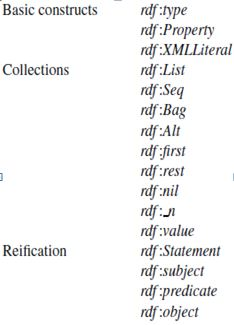
\includegraphics[width=2in]{RDFVocabPic.jpg} 
\caption*{Figure 1: The RDF Vocabulary, from \cite{_social_2007}.}
   \label{}
\label{}   
\end{figure}

\vspace{3mm}
RDF statements consist of triples of the form (subject, predicate, object).  The subject is a resource, either with a URI identifier or a blank identifier.  The predicate is a URI, and the object is either a resource or a literal. Figures 2 and 3 show an example very similar to one in \cite{_social_2007} of an RDF document describing a person named Washington: 

\begin{figure}[h] %  figure placement: here, top, bottom, or page
   \centering
   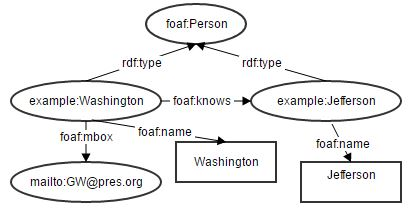
\includegraphics[width=2.5in]{WashJeffPic.jpg} 
\caption*{Figure 2: Example similar to one in \cite{_social_2007}.}
   \label{}
\label{}   
\end{figure}

\vspace{3mm}
\newpage
\begin{itemize}
\item[]@prefix rdfs:  \textless http://www.w3.org/2000/01/rdf-schema\#label\textgreater .
\item[]@prefix rdf:  \textless http://www.w3.org/1999/02/22-rdf-syntax-ns\textgreater .
  \item[]@prefix ex:  \textless http://www.example.org/\textgreater .
  \item[]@prefix foaf:  \textless http://xmlns.com/foaf/0.1/\textgreater .
  \item[] 
  \item[] ex:Washington rdf:type foaf:Person .
 \item[] ex:Jefferson rdf:type foaf:Person .
 \item[] ex:Washington foaf:name "Washington" .
 \item[] ex:Washington foaf:knows example:Jefferson .
 \item[] ex:Washington foaf:mbox \textless mailto:GW@pres.org\textgreater .
 \item[] ex:Jefferson foaf:name "Jefferson" .
\end{itemize}
\begin{center}{Figure 3: Example similar to one in \cite{_social_2007}.}\end{center}
\vspace{3mm}
This example refers to the Friend-of-a-Friend (FOAF) ontology, which is an RDF document on the Web which defines some of the terms used in the example (see\cite{foaf}).  Figure 4 shows some of the FOAF vocabulary.


\begin{figure}[htbp] %  figure placement: here, top, bottom, or page
   \centering
   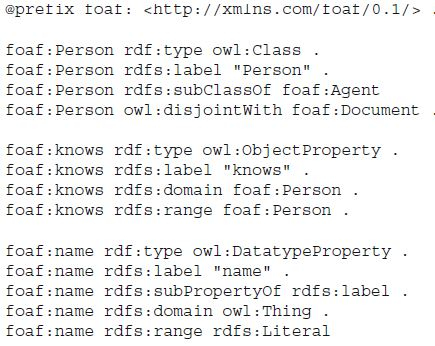
\includegraphics[width=2.5in]{StmtsFromFOAF.jpg} 
  \caption*{Figure 4: Some statements from the FOAF ontology about the terms used in the previous example, taken from \cite{_social_2007}.}
   \label{}
\label{}   
\end{figure}



RDF Schema (RDFs) extends RDF, by including the notion of classes and subclasses.  Domains and ranges of properties are used to connect classes and properties.  Many times RDF and RDFs are referred to interchangeably.  Some RDFs vocabulary is shown in Figure 5.

\begin{figure}[htbp] %  figure placement: here, top, bottom, or page
   \centering
   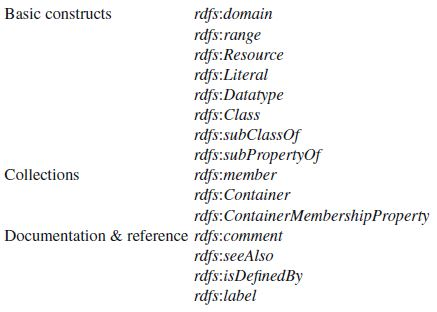
\includegraphics[width=2.5in]{RDFSchemaVocabPic.jpg} 
  \caption*{Figure 5: The RDF Schema Vocabulary, taken from \cite{_social_2007}}
   \label{}
\label{}   
\end{figure}

%\begin{center}{The RDF Schema Vocabulary, taken from \cite{_social_2007}:}\end{center}


RDF(s) uses model-theory semantics , where meaning is defined by mappings from a model to a meta-model in which the truth of propositions is already uniquely determined.  This kind of mapping is called an interpretation, where symbols are mapped to the objects or relations they are describing. Constructs are used to put constraints on possible interpretations, so that unintended interpretations are excluded.  For example, we can use a construct to not allow two symbols used to represent persons to be mapped to the same person.
RDF(s) also allows some axiomatic triples that are true for every model interpretation.  For example, rdfs:subPropertyOf follows the rules shown in Figure 6.

\begin{figure}[htbp] %  figure placement: here, top, bottom, or page
   \centering
   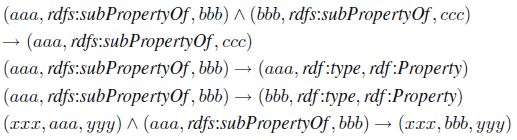
\includegraphics[width=2.8in]{subPropertyOfRules.jpg} 
  \caption*{Figure 6: Example of rdfs:subPropertyOf Rules, from \cite{_social_2007}}
   \label{}
\label{}   
\end{figure}







An important part of RDF semantics is that interpretations are assumed to be open world and monotonic.  An open world assumption means that we can never assume that we have a complete description of the world.  The fact that we have a document describing a certain resource does not imply that we know everything about that resource.  Monotonicity means that new knowledge added is not allowed to make previous references invalid.  As an example, if the range of the foaf:knows property is Person, and we know that a person named Frank knows a dog named Pluto, we don’t take it as a contradiction.  Instead, we assume that there exists some other statement that defines the Dog class to also be in the range of foaf:knows.  That is, statements about an RDF resource only give additional information about that resource and do not invalidate or contradict things previously known about the resource.  

\subsubsection{OWL}
OWL (Web Ontology Language) adds constructs of Description Logics to RDF, which allow for greater expressiveness in characterizing classes and properties.  OWL is really a set of three languages with increasing expressiveness:  OWLLite is a subset of OWLDL which is in turn a subset of OWL Full.  The additional expressivity provided by OWL is used for modelling complex domains like medicine and engineering.

%Peter's picture
\begin{figure*}[t]
\begin{center}
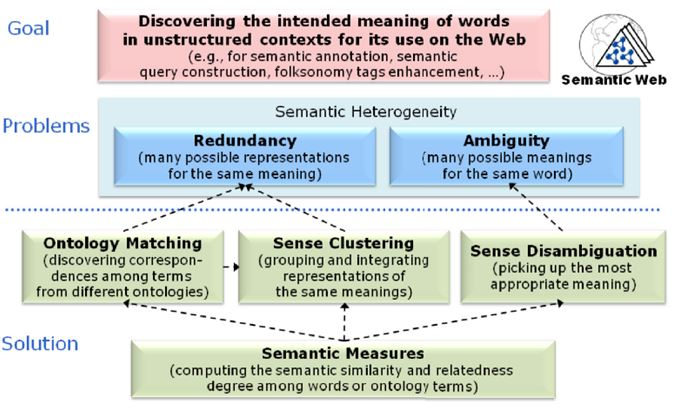
\includegraphics[width=5in]{Peter1.jpg}       
\center\caption*{Figure 7: Dealing with Semantic Heterogeneity, from \cite{gracia_dealing_2011} }
\label{fig1}
\end{center}
\end{figure*}
\subsection{Comparison to Other Formats Commonly Used in Computer Science Domain}
\subsubsection{Comparison to UML}
There is quite a bit of overlap between UML and RDF/OWL.  But UML has a smaller scope because its primitives are for a certain kind of information resource: objects and their roles in an OO system.  So RDF/OWL modelling is less constrained than UML modelling and provides primitives not found in UML, such as the disjointness, union, intersection, and equivalence of classes.

Also, in RDF/OWL , properties are global, and they don’t belong to a class like attributes and associations belong to a certain class in UML.  And non-blank resources in RDF are identified with a URI while UML classes, instances, attributes, etc.,  don’t have such an ID.  And the closed world assumption of UML is of course different from the open world assumption of RDF/OWL.  There are tools available to convert UML class models into OWL ontologies.

\subsubsection{Comparison to E/R Model}
Entity/Relationship modelling is used to model the relations between data structures in database management systems, and is considered as being much simpler than UML.  Entity sets in E/R modelling are roughly like classes in UML.  But in E/R, the only predefined relationship is generalization, which only refers to attribute inheritance; in E/R models, generalization between relationships (ex: subPropertyOf) is not allowed as it is in RDF.  




A useful feature in E/R is the ability to identify keys.  Keys from E/R models can be replicated in RDF/OWL, but composite keys can not.  One advantage that RDF has over E/R modelling is that it gives every resource an identifier, even for resources which are not fully described.  But this disadvantage in E/R modelling can be easily resolved, by creating new primary keys in each entity by making a new column with a unique identifier.

Because many organizations are financially entrenched in their relational databases, it is desirable to keep their data in a RDBMS and map it to a publishable ontology, but this can be difficult in practice.  

\subsubsection{Comparison to XML}
XML and RDF are similar in many aspects.  XML has directed, ordered trees and RDF has directed graphs.  Both XML and RDF are conceptual models having domain specific languages providing their own vocabularies.  But XML is used for representing hierarchical data, with nested, ordered elements.  RDF has a stricter model to represent arbitrary directed graphs with edges representing relationships between classes or instances of classes.  Since there are so many connections between concepts in domain models, hierarchical representations are not sufficient.  While XML has a natural ordering of elements, RDF allows properties to be listed in unconstrained orders.  

\subsection{\textit{Dealing with Semantic Heterogeneity Issues on the Web} \cite{gracia_dealing_2011}}


%Daniela's picture 1
\begin{figure*}[hbt]
\begin{center}
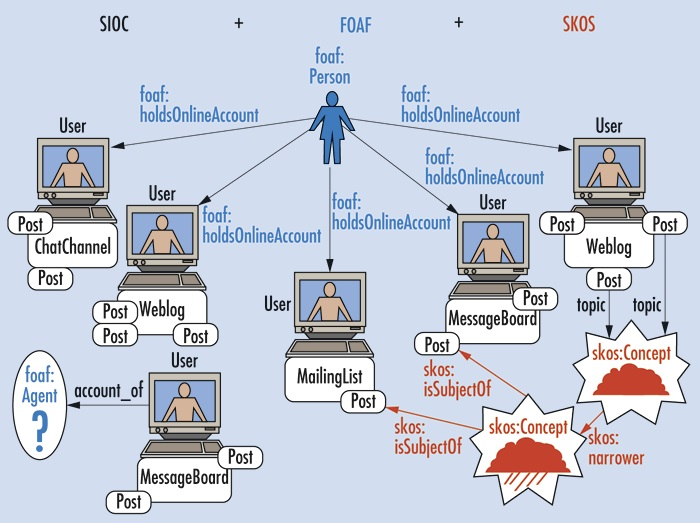
\includegraphics[width=6in]{Daniela1New.JPG}       
\center\caption*{Figure 8: Relationships between Ontologies \cite{6190504} }  
\label{fig1}
\end{center}
\end{figure*}

When working with ontologies, a major concern in the semantic web, there is a hurdle to overcome with the decentralized definition of ontologies. Each individual or organization can define ontologies on their own with no oversight by a central body. This means that the same concept that is defined in one ontology can be defined again in another ontology and may even be defined differently. Another case is that two different ontologies use the same terminology for differing concepts. These two scenarios are defined by Gracia and Mena (\cite{gracia_dealing_2011}) as:
\begin{center} \textbf{Semantic Ambiguity}: many intended meanings are associated with the same word.\end{center}
\begin{center} \textbf{Semantic Redundancy}: many semantic descriptions are available to represent the same intended meaning.\end{center}

An example of this problem is trying to determine the meaning of the word ''apple'' in a query such as ''Give me a list, ordered by calories, of recipes containing apple''. In the example query the term ''apple'' is likely apparent to a human reader, but to a device trying to determine the semantics of the word it can be difficult. If ''apple'' is run through an ontology it might come back with three results, apple the fruit, apple the tree, and Apple the corporation. With these three results the query processor needs to determine what concept represented by ''apple'' does the user want to obtain in the results.

In order to find the correct concept, a search may cross many ontologies where each may have a definition of “apple” and its related concepts. This is where semantic ambiguity and redundancy start to have an effect. In order to filter the search down to likely candidates, word sense disambiguation techniques can be used.

%Daniela's table 1
\begin{figure*}[hbt]
\begin{center}
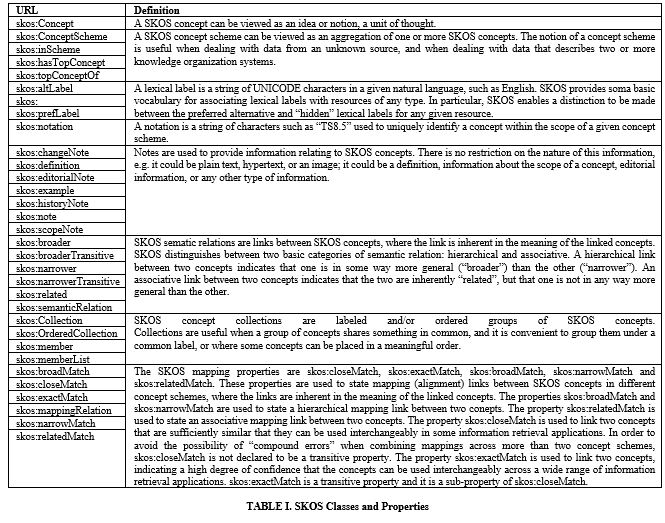
\includegraphics[width=6in]{DanielaTable1.JPG}       
\label{fig1}
\end{center}
\end{figure*}

There are first techniques to reduce semantic heterogeneity of the result set. There are three techniques proposed by Gracia and Mena (\cite{gracia_dealing_2011}) for accomplishing semantic heterogeneity reduction. In ontology matching, a set of terms are compared to each other based on context and the relations that don't meet a threshold are removed. The output of ontology matching then is fed into sense clustering. 

In sense clustering the relatedness of two concepts that share keywords are used to determine if the two concepts should be integrated into a single concept. When two concepts are merged together, then the ontology matching algorithm needs to be run again to calculate the similarities of the new integrated concept.

After sense clustering comes sense disambiguation, in which the concept that the user is trying to query on is determined from the context of the query and the clusters created from sense clustering. This is done by taking the inputted query and breaking it down into keywords and context words to be utilized for the disambiguation and then searching through related concepts in order to find the best fitting one. The first step is to break down the query into individual words and select a keyword and then compute the relatedness of each word to the selected keyword. This works on the assumption that the context with the highest relatedness value is the most likely candidate. The relatedness calculation can be done using something like Normalized Google Distance. With a selected context, the clusters from sense clustering are then weighted within the context to find the likely concept that should be used. The final selection can be done by calculating relatedness, number of word overlaps between concept and context, and determining frequency of appearance of the concept in the context overall. Figure 7 shows a general picture of the authors' ideas.




\subsection{\textit{Using Semantic Web Ontologies for better interoperability on social network sites} \cite{6190504}}
The paper summarized in this section aims at introducing all existing ontologies for semantic web, along with their properties and use in a way to provide a basis for a framework to guarantee inter-operability among multiple social network sites and attain inter-linking of such sites.



%Daniela's table 2
\begin{figure*}[hbt]
\begin{center}
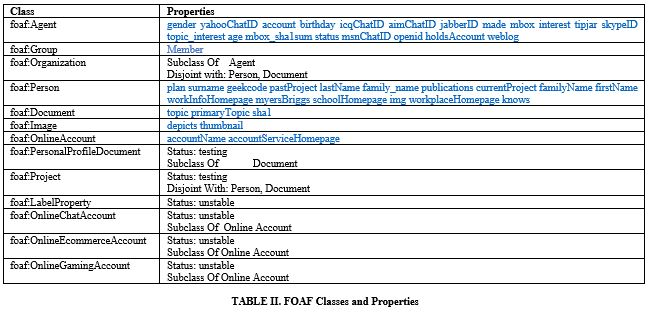
\includegraphics[width=6in]{DanielaTable2.JPG}       
\label{fig1}
\end{center}
\end{figure*}

%Daniela's table 3
\begin{figure*}[hbt]
\begin{center}
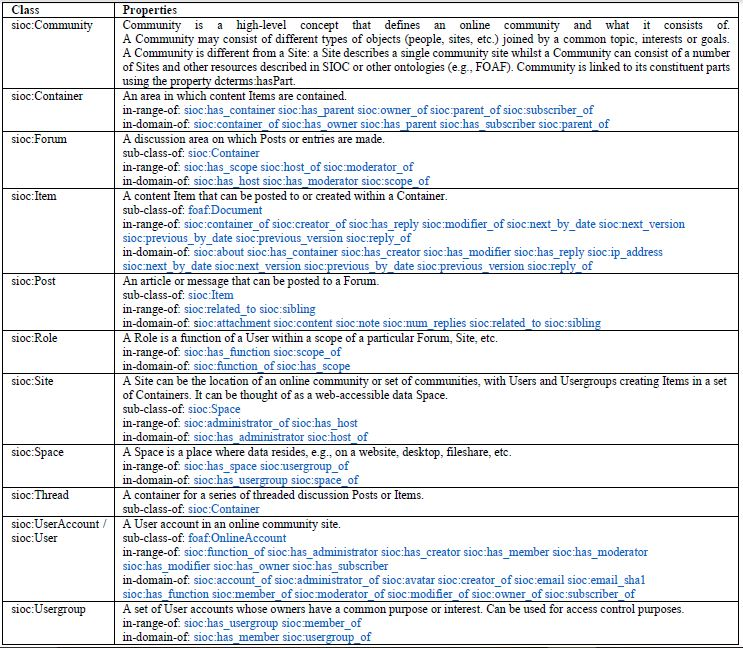
\includegraphics[width=6in]{DanielaTable3.JPG}     
\caption*{\textbf{TABLE III.  SIOC Classes and Properties}}  
\label{fig1}
\end{center}
\end{figure*}

%Daniela's table 4
\begin{figure*}[t]
\begin{center}
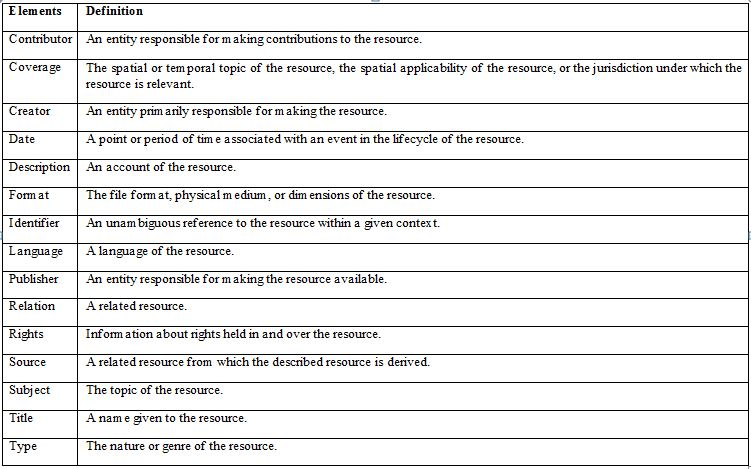
\includegraphics[width=7in]{DanielaTable4.JPG}  
\caption*{\textbf{TABLE IV. Dublin Core (DC) Elements which describe properties of SIOC content items.}}     
\label{fig1}
\end{center}
\end{figure*}



\subsubsection{Problem Introduction}
The authors claim that currently, there are not any established framework that aggregate ontologies. For social networks, which are considered to be ''online networks which indicate connections between actors in social activities'' \cite{6190504}, some interoperability has been reached by the use of ontologies, but no efforts have been done in inter-linking different social network sites. Because of their current isolation, there is a need to expand the potential such networks offer and find new ways of using ontologies to build a better social network environment that could bring forward more relationships among user-generated content in such sites. The studies of semantic web over the years have not proved successful in extracting relationships and integrating social network sites, so the authors propose a framework to be used to address the issue. 



The main challenge of social networks is their inherent nature and the fact that multiple accounts could likely exist for the same user. Furthermore, because of data inconsistency, it is difficult to implement inter-operability and it is also difficult to link multiple social network accounts. Semantic Web was introduced as a technology to make social web sites more connected and to gain more interoperability through metadata creation and inter-connected vocabularies. Existing semantic web vocabulary frameworks such as SIOC (Semantically Interlinked Online Communities) and FOAF (Friend of-a-Friend) could help on this; hence the authors explain multiple vocabularies could be used together to build a good interoperability framework. 

As an example of their use, the authors explain a likely scenario, saying that ''SIOC ontology uses FOAF vocabulary to explore a person’s attributes, and DC (Dublin Core) vocabulary to illustrate SIOC content properties”'' \cite{6190504}. The paper goes on presenting and describing the most dominant and practical ontologies in existence for Semantic Web and how they can be combined to help build an exhaustive framework for social networks; hence proposing a possible solution to the problem.

\subsubsection{Literature Review}
Given the previous definition of social networks, we can see what the impact of using a semantic network can be. According to the authors, '''a semantic network is conceptually a group of entities that are connected through their relationship''' \cite{6190504}. This kind of network provides useful information about individual users that could be used to extract relationships between social network sites. Plainly said, ''Semantic Web is the use of new technologies and standards which allow data interpretation and information processing on the World Wide Web'' \cite{6190504}. Technologies such as RDF (Resource Description Framework) and OWL, can be used in Semantic Web for this purpose. Acquiring related data from social network sites has been challenging, because of the intense amount of data and its varying nature. However, Semantic Web and its technologies such as ontologies and vocabularies have methods for better data presentation and provide the ability for machines to automatically originate data from the web, which is an improvement made possible through these new technologies.






Ontologies are ''tools to analyze and extract relationships among web sites'' \cite{6190504} since as the authors explain, ontologies can ''describe the meaning of a formal vocabulary, identify knowledge within the vocabulary and extract semantics from interconnections on the web'' \cite{6190504}. This capability makes them extremely useful for Semantic Web: they can discover and categorize relationships that exist and delineate relationships between terms within the documents or files that form the Semantic Web Services. 

The four main ontologies and vocabularies extensively employed on the web which are explained in the paper are presented in the list below, the way the authors described them:
\begin{itemize}
\item Dublin Core (DC): It is explained in the paper as a system combining fifteen elements that are used to describe resources. This set of elements assists the search and information retrieval by capturing basic descriptive categories on the web. DC characteristics are: simplicity of creation and maintenance, interoperability among collections and indexing systems, international applicability, extensibility and modularity. These characteristics allow for compiling metadata and creating a mode elaborated description for data resources.

\item Friend of a Friend (FOAF): It is mentioned in the paper that this ontology has been built on top of a RDF based schema to 
''semantically express individuals and their social networks'' \cite{6190504}.

\item Semantically-Interlinked Online Communities (SIOC): It is mentioned to be a Semantic Web technology which has methods that enable interconnection between social network sites (such as Blogs, forums and others). This ontology is an open-standard machine readable format to extract metadata useful for semantic browsing, content management and social web.

\item Simple Knowledge Organization System (SKOS): As expressed in the paper, it is a set of characteristics that provide a standard over RDF documents' vocabularies. Because SKOS can capture organizational knowledge provided in RDF documents, extract similarities and enable technology and information sharing among organization systems, it can be regarded as a ''data model to interlink organization knowledge and facilitate knowledge sharing through the web''\cite{6190504}.


\end{itemize}




Based on the classes and properties related to each ontology, the authors explain that such ontologies can prove to be useful for extracting relationships among diverse social network sites and thus aid in the goal of the paper. Hence, it is the authors' claim that ontologies such as SIOC, FOAF and DC can be combined with other ontologies such as SKOS to obtain more relationships and create a more semantic web.

The classes and properties of each mentioned ontology are shown in TABLE I, TABLE II, TABLE III, and TABLE IV. These tables were taken from the original paper, as well as complemented using sources \cite{skos},\cite{foaf},\cite{sioc}, and \cite{dcmi}. 

\subsubsection{Relationships Among the Ontologies}

Figure 8 also shows the relationships between the four ontologies and it helps explain how to create a framework using them. FOAF documents can be used to describe personal information of social network profiles, which can be enhanced by the use of DC’s elements that in turn would help describe the user’s information more meaningfully. Then, the SIOC ontology can be used to map its classes and properties that describe activities in online social community sites to existing vocabularies such as FOAF, RSS and SKOS. The authors use a common example to illustrate these relationships, saying that the property foaf:Person describes a person who also happens to have different online accounts. Then, the sioc:User class defines the same person on different online community sites. This person/user can create any content on his/her sites by using sioc:Item or post content by using sioc:Post. They are related since the class sioc:User is a sub-class of foaf:OnlineAccount and the property foaf:holdsOnlineAccount is able to link a person to all his/her online accounts. SKOS classes and properties such as skos:Concept and skos:isSubjectOf describe the contents of the posts and the information itself within the user’s online accounts. Therefore, the three ontologies (SIOC, FOAF and SKOS) can be used together in collaboration to produce an integrated framework.


In the authors' opinion, the related classes and properties of the discussed semantic web ontologies would help build a holistic framework that can describe user-generated content in social network sites and connect them appropriately. They propose that the use of FOAF can help define multiple accounts in social network sites belonging to the same user, which would allow for SIOC to articulate user-content on the sites. Then by using SKOS, it would be possible to define the most related ontology to each user-content and tag it appropriately.

However, the authors only explored the current ontology technologies and their possible interaction to build the mentioned framework, but neither implemented such framework nor tested it empirically on social network sites to see whether it achieved the goals of creating more connectivity and having a better user content management system. They mentioned further work was necessary to convert the theoretical framework into a practical one.









\section{Conclusion}
Based on the resources analyzed we have seen that the semantic web is still growing and evolving and eventually will allow for an interconnected web of social networks. The research we reviewed, did not provide an implementation but did describe how these technologies, methods, and concepts can be applied together to create a more connected and machine friendly web. The reach of semantic web goes far beyond social networks and we only scratched the surface of one area of its application and usefulness.


\section{Future Work}
\begin{itemize}
\item
A common framework RDFs/OWL that can be used to generalize and relate social networks to each other so that users can be identified across networks.
\item
A means of linking users across social networks and then consolidating their content so that the user and their content as a whole can be queried.
\item
A means of detecting a user being a member of multiple social networking sites and linking those multiple accounts to one resource by filtering out users that share similar attributes and identifying characteristics.
\end{itemize}

%
%To cite the chapter from Mahmood: \cite{_social_2007}  \\
%To cite Peter's paper: \cite{gracia_dealing_2011} \\
%To cite Daniela's paper: \cite{6190504} \\
%To cite sioc: \cite{sioc} \\
%To cite foaf: \cite{foaf} \\
%To cite dcmi: \cite{dcmi} \\
%To cite skos: \cite{skos}


\newpage

\bibliography{MyLibrary} 
\nocite{*}
\bibliographystyle{ieeetr}


\end{document}
